\section{Hadoop 2.2}
\label{sec:hadoop-2.2}

\par A partir des versions , Hadoop vient avec un nouveau composant appelé Yarn. 

\begin{figure}[h!]
  \centering
  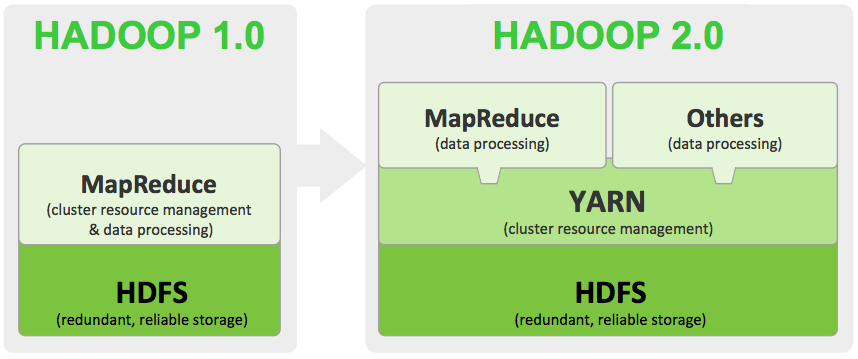
\includegraphics[width=12cm]{images/yarn.png}
  \caption{Différences entre Hadoop 1.x et Hadoop 2.x}
  \label{fig:yarn}
\end{figure}

Yarn est responsable de la gestion des ressources, et utilise des processus similaires pour leur gestion. Le NodeManager vient remplacer le TaskTracker, qui s'occupe de faire le lien entre le DataNode et le ResourceManager localisé sur le master (NameNode). Le ResourceManager déploie les applications sur les noeuds grâce à sa communication avec les NodeManagers.

\subsection{Connexion sur un ordinateur à Supélec}
\label{sec:connexion-sur-un}

\par La connexion avec un compte utilisateur précis est particulière, dans la mesure où on peut accéder à son dossier personnel, correspondant à des identifiants de connexion, depuis n'importe quelle machine. En effet, une machine est responsable de la gestion des logins, et contient les données personnelles correspondantes. Ces données transitent lors d'une connexion, ce qui peut faire croire que ces données sont présentes sur tous les ordinateurs.

\par Il est important de garder à l'esprit ce mécanisme, car c'est grâce à celui-ci que nous pourront simplifier la configuration de Hadoop sur le cluster Skynet. Malgré ces données qui ne sont pas propres à une machine, nous devons également pouvoir accéder à la mémoire de la machine physique, afin de pouvoir les utiliser comme DataNodes. Dans un premier temps, nous utiliserons le dossier \texttt{/tmp} accessible en lecture écriture à n'importe qui (donc peu sécurisé, mais adapté à notre installation de test).

\begin{figure}[h!]
  \centering
  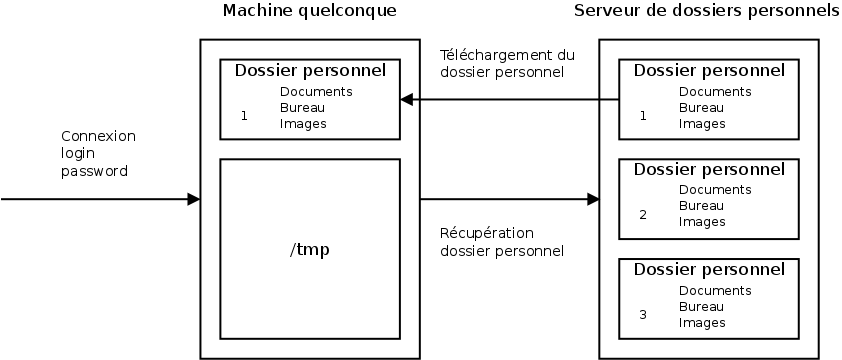
\includegraphics[width=16cm]{images/connexion_supelec.png}
  \caption{Exemple d'une connexion sur une machine quelconque}
  \label{fig:connexion_supelec}
\end{figure}

\subsection{Connexion SSH}
\label{sec:connexion-ssh}

\par Lors d'une connexion SSH, le fichier \texttt{.bash\_profile} est executé. Lors d'un login, c'est le fichier \texttt{.bashrc} qui est exécuté. Comme toutes les connexions via hadoop se font par ssh, nous allons les lier tous les deux. Pour cela, on créera un fichier \texttt{.bash\_profile} contenant au moins :

\begin{minted}[frame=single,linenos,mathescape]{bash}
  if [ -f .bashrc ]; then
    . ~/.bashrc
  fi
\end{minted}

\par De cette manière, si le fichier \texttt{.bashrc} existe, on le charge, sinon on ne fait rien.
\par On se connecte successivement sur \texttt{Ghome}, puis \texttt{Term2} :
\begin{minted}[frame=single,linenos,mathescape]{bash}
  Alex > ssh ghome
  Last login: Sat Jun 14 22:00:38 2014 from 193.48.225.99
  Alex [gserver] > ssh term2
  Last login: Sat Jun 14 20:52:34 2014 from gserver.grid.metz.supelec.fr
  Alex [term2] > 
\end{minted}

\par A partir de \texttt{Term2}, on peut se connecter à chacune des machines du cluster Skynet, dont les alias permettent de simplifier les opérations. Ainsi au lieu de 

\begin{minted}{bash}
  ssh careil_ale@term2.grid.metz.supelec.fr
\end{minted}
 on peut simplement faire
\begin{minted}{bash}
  ssh careil_ale@term2
\end{minted}

car nous sommes dans le domaine \texttt{grid.metz.supelec.fr}.

 Il est inutile de spécifier le nom d'utilisateur lors de la connexion puisque, comme expliqué précédemment, notre compte existe sur toutes les machines (pas physiquement, mais il est chargé à chaque fois). Donc au lieu de se connecter avec la commande précédente, on peut simplement faire :
 
\begin{minted}{bash}
  ssh term2
\end{minted}

Cependant, il faut effectuer une manoeuvre afin de pouvoir se connecter facilement sans mot de passe. En effet, on va générer une clé SSH avec la commande \texttt{ssh-keygen} (qu'on appellera \texttt{id\_rsa\_test}). Vu qu'on ne veut pas utiliser de mot de passe pour se connecter, on omettra la \texttt{Passphrase} lors de la création de la clé.

\begin{verbatim}
Alex > ssh-keygen
Generating public/private rsa key pair.
Enter file in which to save the key (/home/alexandre/.ssh/id_rsa): id_rsa_test
Enter passphrase (empty for no passphrase): 
Enter same passphrase again: 
Your identification has been saved in id_rsa_test.
Your public key has been saved in id_rsa_test.pub.
The key fingerprint is:
61:e0:38:43:34:aa:fc:7b:6e:e3:04:79:a2:f6:14:1a alexandre@gentooalex
The key's randomart image is:
+--[ RSA 2048]----+
|   .+ .          |
|   o + .         |
|  . + . o        |
|..  .o . .       |
|.E = .  S        |
|  = =            |
| + o .           |
|. o o+           |
|   o=o.          |
+-----------------+
\end{verbatim}

\par Maintenant, allons dans le dossier \texttt{.ssh} contenant notre clé publique, et notre clé privée afin de créer le fichier \texttt{authorized\_keys} s'il n'existe pas déjà. S'il n'existe pas, tapez la commande \texttt{touch authorized\_keys} afin de le créer.

\par On va ajouter notre clé publique à l'ensemble des clés autorisées :
\begin{verbatim}
cat id_rsa_test.pub >> authorized_keys
\end{verbatim}
\par On peut désormais vérifier que cela fonctionne bien en se connectant par exemple à \texttt{sh00}. Normalement, aucun mot de passe n'est demandé. 

\par Un dernier problème peut empêcher une connexion directe en ssh, celui de la vérification d'authenticité de l'hôte sur lequel on veut se connecter : 
\begin{verbatim}
Juan [master] > ssh munozperez_jua@ghomE.metz.supelec.fr
The authenticity of host 'ghome.metz.supelec.fr (193.48.224.129)' 
can't be established.
RSA key fingerprint is c1:41:c3:6d:f1:21:a2:2a:e6:30:b0:60:f7:de:22:b1.
Are you sure you want to continue connecting (yes/no)? YES
Warning: Permanently added 'ghome.metz.supelec.fr,193.48.224.129' 
(RSA) to the list of known hosts.
Last login: Sun Apr  6 21:20:11 2014 from 193.48.225.99
\end{verbatim}

\par Pour enlever ce message, il faut se connecter manuellement à chaque noeud pour qu'il soit ajouté à la liste des hôtes connus (listés dans le fichier \texttt{~/.ssh/known\_hosts}).

\subsection{Hadoop avec OAR}
\label{sec:hadoop-avec-oar}

\par On prévoit d'utiliser Hadoop avec OAR. C'est-à-dire qu'une fois connecté sur \texttt{Term2}, on effectue une requête \texttt{OAR} en intéractif afin de commander des noeuds sur le cluster (Skynet dans notre cas). Si la requête se solde par un succès, une session est ouverte (une connexion ssh...) sur le noeud qui va nous permettre de les utiliser tous.

\par Ce n'est qu'une fois la session lancée qu'on peut commencer à configurer Hadoop ! D'où l'intérêt d'automatiser la génération de ces fichiers en fonction de la session, des noeuds commandés... 
\par Typiquement, le noeud sur lequel on arrive sera le \texttt{NameNode}, et générera les fichiers de configuration pour tous les noeuds (master et slave).

\par Pour générer les fichiers de configuration de manière automatisée, on va créer des fichiers contenant des variables telles que le nom du \texttt{NameNode} (que l'on connaît grâce à la variable \texttt{HADOOP\_NAMENODE\_NAME} par exemple). Ces fichiers seront placés dans un dossier \texttt{hadoop\_conf\_original}, et permettront de générer à chaque session \texttt{OAR} des fichiers de configuration adaptés à la session en cours (avec le nom du \texttt{NameNode}, \texttt{SecondaryNameNode}...). Grâce à la variable \texttt{OAR\_FILE\_NODE}, on obtient le nom des machines que l'on a réservées avec \texttt{OAR}.

\newpage

\subsection{Création des fichiers de configuration de Hadoop}
\label{sec:creat-des-fich}

\subsubsection{.bashrc}
\label{sec:.bashrc}

\par Ce fichier va nous permettre d'instancier des variables d'environnement utiles pour Hadoop au moment d'une connexion SSH. Comme expliqué précédemment, c'est le fichier \texttt{.bash\_profile} qui est chargé, mais nous ferons en sorte que ce dernier fasse appel au \texttt{.bashrc}, dont nous allons donc détailler le contenu.

\paragraph{Variables d'environnement utilisées par Hadoop}
\label{sec:vari-denv-util}

\begin{minted}[frame=single,linenos,mathescape]{bash}
export JAVA_HOME=/usr/lib/jvm/java

# Hadoop
HADOOP_PREFIX=/opt/hadoop-2.2.0
export HADOOP_HOME=$HADOOP_PREFIX
export HADOOP_COMMON_HOME=$HADOOP_PREFIX
export HADOOP_HDFS_HOME=$HADOOP_PREFIX
export HADOOP_MAPRED_HOME=$HADOOP_PREFIX
export HADOOP_YARN_HOME=$HADOOP_PREFIX
export PATH=$PATH:$HADOOP_HOME/bin:$HADOOP_HOME/sbin

export HADOOP_COMMON_LIB_NATIVE_DIR=${HADOOP_PREFIX}"/lib/native/"
export HADOOP_OPTS="${HADOOP_OPTS}
 -Djava.library.path=$HADOOP_PREFIX/lib/"

export HADOOP_CONF_DIR=~/hadoop_conf
export HADOOP_LOG_DIR=~/hadoop_logs
export HADOOP_NAMENODE_NAME=localhost
\end{minted}

\par Dans cette première partie, nous définissons la variable \texttt{JAVA\_HOME} nécessaire pour localiser la machine virtuelle Java à utiliser pour exécuter Hadoop, qui, rappelons le, est codé en Java. Généralement, sous Linux, le chemin à mettre est très simple, car il s'agit d'un lien symbolique (l'adresse ne pointe donc pas directement sur la bonne version de Java à utiliser, mais sur un "fichier lien" qui pointe sur la version actuelle de Java utilisée sur le système).

\par \texttt{HADOOP\_PREFIX} est une variable "maison" nous permettant de ne spécifier le chemin vers Hadoop une seule fois. De cette manière, si on devait changer Hadoop d'emplacement, la modification de cette variable seule nous permettrait de modifier toutes les autres. Elle n'est donc pas utilisée par Hadoop.

\par \texttt{HADOOP\_HOME}, \texttt{HADOOP\_COMMON\_HOME},
\texttt{HADOOP\_HDFS\_HOME}, \texttt{HADOOP\_MAPRED\_HOME}, \\ \texttt{HADOOP\_YARN\_HOME}, sont les variables de base, spécifiant les chemins vers les divers composants de Hadoop. Dans notre cas, l'installation simple réunit tous les composants au même endroit, mais ce n'est pas tout le temps le cas. On les fixe donc toutes à \texttt{HADOOP\_PREFIX}.

\par La variable \texttt{PATH} est utilisée par le Shell (bash dans notre cas) afin de faire correspondre chaque commande tapée avec un programme localisé dans un des dossiers spécifiés dans cette variable. Par défaut, on a généralement \texttt{PATH=/bin:/usr/bin:/usr/local/bin}, car les programmes installés par défaut (de type interne comme par exemple \texttt{ls}, \texttt{cat}... ) sont installés dans \texttt{/bin}. Ceux installés par l'utilisateur sont localisés dans \texttt{/usr/bin}. Les programmes nécessitant des privilèges administrateurs pour être exécutés sont dans \texttt{/usr/sbin}, et ce dossier n'est ajouté à la variable \texttt{PATH} que lorsqu'on est connecté avec le compte administrateur \texttt{root}.

\par Les variables \texttt{HADOOP\_OPTS} et \texttt{HADOOP\_COMMON\_LIB\_NATIVE} permettent de spécifier respectivement le dossier dans lequel Java doit aller chercher les librairies (compilées car écrites en \texttt{C}), et le dossier contenant les librairies natives (ces mêmes librairies, mais compilées spécifiquement pour la machine sur laquelle Hadoop est exécuté).

\par \texttt{HADOOP\_CONF\_DIR} permet de spécifier l'emplacement des fichiers de configuration de Hadoop, chose très importante dans notre cas puisque nous les localisons dans notre espace personnel, afin qu'ils soient accessibles à chaque connexion ssh, quelque soit la machine.

\par \texttt{HADOOP\_LOG\_DIR} redéfinit par défaut le dossier dans lequel les logs relatifs aux composants Hadoop (\texttt{NameNode}, \texttt{SecondaryNameNode} et \texttt{DataNode} sont stockés. Il est indispensable de les localiser sur notre espace personnel (\texttt{~/.}), d'une part pour des questions de droits d'écriture, car le dossier \texttt{/opt/hadoop-2.2.0} n'est actuellement pas accessible en écriture pour les utilisateurs lambda, et d'autre part car si plusieurs utilisateurs venaient à utiliser Hadoop, les logs générés seraient alors centralisés, et rendrait leur consultation difficile.

\par La dernière variable de cet extrait de \texttt{.bashrc} est une variable qui nous sera utile par la suite. \texttt{HADOOP\_NAMENODE\_NAME} contient en fait le nom de la machine qui fait office de NameNode.

\paragraph{Configuration du prompt}
\label{sec:conf-du-prompt}

\par La configuration du prompt va nous permettre de naviguer plus efficacement de machine en machine. En effet, par défaut, le prompt ressemble à \texttt{bash4.2\$ }, ce qui n'est pas très utile en soit. Il serait plus intéressant d'avoir le nom d'hôte de la machine sur laquelle on est connecté.


\begin{minted}[frame=single,linenos,mathescape]{bash}
case "$TERM" in
"dumb")
    export PS1="> "
    ;;
xterm*|rxvt*|eterm*|screen*)
    export PS1='\[\033[00;32m\]Alex [\h] > \[\033[00m\]'
    ;;
*)
    export PS1="> "
    ;;
esac
\end{minted}

\par La variable d'environnement \texttt{TERM} permet de spécifier le type de terminal utilisé. Chaque émulateur de terminal initialise cette variable selon son nom généralement. Par exemple, si on utilise \texttt{xterm}, on aura \texttt{TERM=xterm}. 
\par Changer le prompt peut nous faciliter la vie lorsqu'on utilise un terminal comme \texttt{xterm} ou \texttt{rxvt}, mais on peut par exemple utiliser un autre logiciel qui se connecte en ssh en parsant le prompt, comme l'extension \texttt{TRAMP} d'Emacs. Si le prompt est différent de \texttt{ >}, la connexion sera impossible. Et plus généralement, il vaut mieux garder un prompt simple et standard pour toutes les autres utilisations potentielles. C'est ainsi que notre \texttt{switch} intervient. Selon la valeur la valeur de \texttt{TERM}, on redéfinit la variable \texttt{PS1} qui contient le prompt de manière plus ou moins standard.

\paragraph{Construction du NameNode}
\label{sec:constr-du-namen}

\par Une fois la requête \texttt{OAR} effectuée, nous arrivons sur un noeud sur lequel des variables d'environnement \texttt{OAR} sont instanciées. C'est de cette manière qu'on identifiera le \texttt{NameNode}, car les autres noeuds n'ont pas ces variables.

\begin{minted}[frame=single,linenos,mathescape]{bash}
if [ ! -d "/tmp/hadoop-tmp" ]; then mkdir /tmp/hadoop-tmp; fi
if [ ! -d "/tmp/hadoop-tmp/hdfs" ]; then mkdir /tmp/hadoop-tmp/hdfs; fi
if [ ! -d "/tmp/hadoop-tmp/hdfs/datanode" ]; then
    mkdir /tmp/hadoop-tmp/hdfs/datanode;
fi
# Si on est sur le NameNode
if [ -n "$OAR_FILE_NODES" ]; then
    if [ ! -d "/tmp/hadoop-tmp/hdfs/namenode" ]; then
        mkdir /tmp/hadoop-tmp/hdfs/namenode;
    fi
    if [ ! -d "/tmp/hadoop-tmp/hdfs/namesecondary" ]; then
        mkdir /tmp/hadoop-tmp/hdfs/namesecondary;
    fi
    
    # Si le dossier de configuration n'existe pas on le crée
    if [ ! -d "$HADOOP_CONF_DIR" ]; then 
        mkdir $HADOOP_CONF_DIR;
    # sinon on le vide
    else rm -f $HADOOP_CONF_DIR"/*";
    fi
    if [ ! -d $HADOOP_CONF_DIR"_slaves" ]; then
	mkdir $HADOOP_CONF_DIR"_slaves";
    else rm -f $HADOOP_CONF_DIR"_slaves/*";
    fi

    # Définition du nom du Namenode
    export HADOOP_NAMENODE_NAME=$(head -1 $OAR_FILE_NODES);
    for f in ~/hadoop_conf_original/*; do
	cat $f | sed -e \ 
	's/\$HADOOP_NAMENODE_NAME/'$HADOOP_NAMENODE_NAME'/g' \ 
	> ~/hadoop_conf/$(basename $f);
    done;
    cat $OAR_FILE_NODES | uniq > $HADOOP_CONF_DIR/slaves;
    for f in ~/hadoop_conf_slaves_original/*; do
	cat $f | sed  \ 
	-e 's/\$HADOOP_NAMENODE_NAME/'$HADOOP_NAMENODE_NAME'/g' \ 
	> ~/hadoop_conf_slaves/$(basename $f);
    done;
else
    export HADOOP_CONF_DIR=~/hadoop_conf_slaves;
fi
\end{minted}

\par Expliquons donc ce gros morceau de code \texttt{bash}. On commence par créer s'ils n'existent pas, les dossiers sur la machine physique qui vont permettre de stocker les données. On suppose que toute machine est un \texttt{DataNode}, donc on créera d'abord le dossier \texttt{/tmp/hadoop-tmp}, puis dedans on créera un dossier \texttt{hdfs}, avant de finalement créer le dossier \texttt{datanode} qui contiendra les données du \texttt{DataNode}.
\par Si on se connecte sur le \texttt{NameNode}, ce que l'on sait en vérifiant l'existence de la variable \texttt{OAR\_NODE\_FILE}, on ajoute deux dossiers supplémentaires \texttt{namenode} et \texttt{namesecondary}, respectivement pour le \texttt{NameNode} et le \mathtt{SecondaryNameNode}.
\par Une fois ces dossiers créés sur la machine physique (c'est-à-dire que si on se connecte sur une autre machine, ces dossiers n'apparaîtront pas), on crée les dossiers sur l'espace personnel qui vont accueillir les fichiers de configuration générés. Donc s'ils n'existent pas, on crée les dossiers \texttt{hadoop\_conf} et \texttt{~/hadoop\_conf\_slaves}, et s'ils existent déjà, c'est qu'ils ont probablement déjà accueilli des fichiers de configuration lors d'une précédente session \texttt{OAR}, dans ce cas on les vide.
\par Dernière étape, lors de la connexion sur le \texttt{NameNode}, on génère les fichiers de configuration qui vont être utilisés !
Pour cela, on redéfinit la variable \texttt{HADOOP\_NAMENODE\_NAME} en prenant le premier nom d'hôte dans la liste des hôtes fournis, accessible via la commande \texttt{cat \$OAR\_FILE\_NODE}. En fait, les variables \texttt{bash} ne sont pas évaluées dans les fichiers de configuration \texttt{xml} de Hadoop, d'où la nécessité d'en générer de nouveaux, avec les références au \texttt{NameNode} en dur. On crée donc chaque fichier à partir de son original, aussi bien pour \texttt{hadoop\_conf} que pour \texttt{hadoop\_conf\_slaves}, en remplaçant \texttt{HADOOP\_NAMENODE\_NAME} par sa valeur. Pour le dossier \texttt{hadoop\_conf}, on met à jour le fichier \texttt{slaves} grâce au contenu du fichier désigné par la variable \texttt{OAR\_FILE\_NODE}.

\par Pour finir, si on se connecte sur un autre noeud que le \texttt{NameNode}, en supposant qu'il s'agisse d'un noeud qui ne possède pas de variables d'environnement \texttt{OAR}, on change simplement la variable \texttt{HADOOP\_CONF\_DIR} afin qu'elle pointe vers les fichiers de configuration du dossier \texttt{hadoop\_conf\_slaves}, spécifiques aux machines esclaves. Nous concernant, à part le fichier \texttt{slaves} qui diffère entre les deux dossiers, tous les autres fichiers sont identiques, il ne s'agit donc que d'une pure précaution dans le cas où il faudrait spécifier des configurations différentes pour les maîtres et les esclaves.

\paragraph{Précautions lors de la déconnexion}
\label{sec:precautions-lors-de}

\par Lorsque sur une session \texttt{OAR} les services Hadoop sont démarrés, il est dangereux de se déconnecter sans les arrêter. Arrêter la session \texttt{OAR} avant d'avoir arrêté Hadoop mène tout droit à un encombrement des ports. En effet, chaque composant de Hadoop utilise un port spécifié dans les fichiers de configuration, et si on quitte la session \texttt{OAR} avant d'arrêter les services, ceux-ci restent occupés et cela empêche Hadoop de se lancer correctement la fois suivante (sauf si les machines ont subi un reboot entre temps).

\par On se propose, pour éviter toute déconnexion hasardeuse lorsque des services seraient encore actifs, d'afficher un message de confirmation au moment de la déconnexion. Ce message ne s'afficherait que si le nombre de processus Java lancés est supérieur ou égal à 1. On voit les processus grâce à la commande \texttt{jps}. Cette commande retourne au moins une ligne, correspondant au processus \texttt{Jps}. Si le nombre de lignes retournées par cette commande est strictement supérieur à 1, il y a des processus Java lancés, et le message de confirmation s'affiche.

\par Pour ce faire, on utilise une fonction auxiliaire (dont l'idée appartient à un bloggeur) \texttt{confirm} qui retourne une erreur \texttt{1} si on ne répond pas \texttt{yes}, et bloque la suite des opérations. En combinant cette fonction avec la commande \texttt{exit}, à l'aide de l'opérateur \texttt{&&}, si la fonction \texttt{confrm} ne s'exécute pas correctement (si on n'a pas répondu \texttt{yes}), la commande placée après ne s'exécute pas.
\begin{verbatim}
confirm Logout ? && exit;
\end{verbatim}

\par En ayant connaissance de cette astuce, on crée donc la fonction testExit qui va tester le nombre de lignes retournées par \texttt{jps}, et on le prend supérieur strictement à 1. Sinon on ne met pas de message de confirmation.
\begin{minted}[frame=single,linenos,mathescape]{bash}
function confirm()
{
    echo -n "$@ "
    read -e answer
    for response in y Y yes YES Yes Sure sure SURE OK ok Ok
    do
        if [ "_$answer" == "_$response" ]
        then
            return 0
        fi
    done
 
    # Any answer other than the list above is considerred a "no" answer
    return 1
}

function testExit()
{
    if [[ "$(jps|wc -l)" -gt "1" ]]; then
	confirm Avez-vous bien arrêté tous les processus Java ?\ 
        \(commande jps\) yes/no && logout;
    else
	logout;
    fi
}

alias exit="testExit";
\end{minted}

\par Note concernant l'utilisation de \texttt{logout} : on n'utilise pas la fonction \texttt{exit} dans la déclaration de \texttt{testExit}, car l'idée est de définir exit comme alias de cette fonction. Donc si on appelait \texttt{exit} dans \texttt{testExit}, elle s'appellerait à l'infini, d'où l'astuce du \texttt{logout}.

%%% Local Variables: 
%%% mode: latex
%%% TeX-master: "CompteRendu"
%%% End: 
